\documentclass[]{article}
\usepackage{lmodern}
\usepackage{amssymb,amsmath}
\usepackage{ifxetex,ifluatex}
\usepackage{fixltx2e} % provides \textsubscript
\ifnum 0\ifxetex 1\fi\ifluatex 1\fi=0 % if pdftex
  \usepackage[T1]{fontenc}
  \usepackage[utf8]{inputenc}
\else % if luatex or xelatex
  \ifxetex
    \usepackage{mathspec}
  \else
    \usepackage{fontspec}
  \fi
  \defaultfontfeatures{Ligatures=TeX,Scale=MatchLowercase}
\fi
% use upquote if available, for straight quotes in verbatim environments
\IfFileExists{upquote.sty}{\usepackage{upquote}}{}
% use microtype if available
\IfFileExists{microtype.sty}{%
\usepackage{microtype}
\UseMicrotypeSet[protrusion]{basicmath} % disable protrusion for tt fonts
}{}
\usepackage[margin=1in]{geometry}
\usepackage{hyperref}
\hypersetup{unicode=true,
            pdftitle={Lab1-R},
            pdfauthor={Clayton Glenn},
            pdfborder={0 0 0},
            breaklinks=true}
\urlstyle{same}  % don't use monospace font for urls
\usepackage{color}
\usepackage{fancyvrb}
\newcommand{\VerbBar}{|}
\newcommand{\VERB}{\Verb[commandchars=\\\{\}]}
\DefineVerbatimEnvironment{Highlighting}{Verbatim}{commandchars=\\\{\}}
% Add ',fontsize=\small' for more characters per line
\usepackage{framed}
\definecolor{shadecolor}{RGB}{248,248,248}
\newenvironment{Shaded}{\begin{snugshade}}{\end{snugshade}}
\newcommand{\KeywordTok}[1]{\textcolor[rgb]{0.13,0.29,0.53}{\textbf{#1}}}
\newcommand{\DataTypeTok}[1]{\textcolor[rgb]{0.13,0.29,0.53}{#1}}
\newcommand{\DecValTok}[1]{\textcolor[rgb]{0.00,0.00,0.81}{#1}}
\newcommand{\BaseNTok}[1]{\textcolor[rgb]{0.00,0.00,0.81}{#1}}
\newcommand{\FloatTok}[1]{\textcolor[rgb]{0.00,0.00,0.81}{#1}}
\newcommand{\ConstantTok}[1]{\textcolor[rgb]{0.00,0.00,0.00}{#1}}
\newcommand{\CharTok}[1]{\textcolor[rgb]{0.31,0.60,0.02}{#1}}
\newcommand{\SpecialCharTok}[1]{\textcolor[rgb]{0.00,0.00,0.00}{#1}}
\newcommand{\StringTok}[1]{\textcolor[rgb]{0.31,0.60,0.02}{#1}}
\newcommand{\VerbatimStringTok}[1]{\textcolor[rgb]{0.31,0.60,0.02}{#1}}
\newcommand{\SpecialStringTok}[1]{\textcolor[rgb]{0.31,0.60,0.02}{#1}}
\newcommand{\ImportTok}[1]{#1}
\newcommand{\CommentTok}[1]{\textcolor[rgb]{0.56,0.35,0.01}{\textit{#1}}}
\newcommand{\DocumentationTok}[1]{\textcolor[rgb]{0.56,0.35,0.01}{\textbf{\textit{#1}}}}
\newcommand{\AnnotationTok}[1]{\textcolor[rgb]{0.56,0.35,0.01}{\textbf{\textit{#1}}}}
\newcommand{\CommentVarTok}[1]{\textcolor[rgb]{0.56,0.35,0.01}{\textbf{\textit{#1}}}}
\newcommand{\OtherTok}[1]{\textcolor[rgb]{0.56,0.35,0.01}{#1}}
\newcommand{\FunctionTok}[1]{\textcolor[rgb]{0.00,0.00,0.00}{#1}}
\newcommand{\VariableTok}[1]{\textcolor[rgb]{0.00,0.00,0.00}{#1}}
\newcommand{\ControlFlowTok}[1]{\textcolor[rgb]{0.13,0.29,0.53}{\textbf{#1}}}
\newcommand{\OperatorTok}[1]{\textcolor[rgb]{0.81,0.36,0.00}{\textbf{#1}}}
\newcommand{\BuiltInTok}[1]{#1}
\newcommand{\ExtensionTok}[1]{#1}
\newcommand{\PreprocessorTok}[1]{\textcolor[rgb]{0.56,0.35,0.01}{\textit{#1}}}
\newcommand{\AttributeTok}[1]{\textcolor[rgb]{0.77,0.63,0.00}{#1}}
\newcommand{\RegionMarkerTok}[1]{#1}
\newcommand{\InformationTok}[1]{\textcolor[rgb]{0.56,0.35,0.01}{\textbf{\textit{#1}}}}
\newcommand{\WarningTok}[1]{\textcolor[rgb]{0.56,0.35,0.01}{\textbf{\textit{#1}}}}
\newcommand{\AlertTok}[1]{\textcolor[rgb]{0.94,0.16,0.16}{#1}}
\newcommand{\ErrorTok}[1]{\textcolor[rgb]{0.64,0.00,0.00}{\textbf{#1}}}
\newcommand{\NormalTok}[1]{#1}
\usepackage{graphicx,grffile}
\makeatletter
\def\maxwidth{\ifdim\Gin@nat@width>\linewidth\linewidth\else\Gin@nat@width\fi}
\def\maxheight{\ifdim\Gin@nat@height>\textheight\textheight\else\Gin@nat@height\fi}
\makeatother
% Scale images if necessary, so that they will not overflow the page
% margins by default, and it is still possible to overwrite the defaults
% using explicit options in \includegraphics[width, height, ...]{}
\setkeys{Gin}{width=\maxwidth,height=\maxheight,keepaspectratio}
\IfFileExists{parskip.sty}{%
\usepackage{parskip}
}{% else
\setlength{\parindent}{0pt}
\setlength{\parskip}{6pt plus 2pt minus 1pt}
}
\setlength{\emergencystretch}{3em}  % prevent overfull lines
\providecommand{\tightlist}{%
  \setlength{\itemsep}{0pt}\setlength{\parskip}{0pt}}
\setcounter{secnumdepth}{0}
% Redefines (sub)paragraphs to behave more like sections
\ifx\paragraph\undefined\else
\let\oldparagraph\paragraph
\renewcommand{\paragraph}[1]{\oldparagraph{#1}\mbox{}}
\fi
\ifx\subparagraph\undefined\else
\let\oldsubparagraph\subparagraph
\renewcommand{\subparagraph}[1]{\oldsubparagraph{#1}\mbox{}}
\fi

%%% Use protect on footnotes to avoid problems with footnotes in titles
\let\rmarkdownfootnote\footnote%
\def\footnote{\protect\rmarkdownfootnote}

%%% Change title format to be more compact
\usepackage{titling}

% Create subtitle command for use in maketitle
\newcommand{\subtitle}[1]{
  \posttitle{
    \begin{center}\large#1\end{center}
    }
}

\setlength{\droptitle}{-2em}
  \title{Lab1-R}
  \pretitle{\vspace{\droptitle}\centering\huge}
  \posttitle{\par}
  \author{Clayton Glenn}
  \preauthor{\centering\large\emph}
  \postauthor{\par}
  \predate{\centering\large\emph}
  \postdate{\par}
  \date{January 18, 2018}


\begin{document}
\maketitle

\section{Tasks}\label{tasks}

\subsection{Task 1}\label{task-1}

\subsubsection{Get Working Directory}\label{get-working-directory}

\begin{Shaded}
\begin{Highlighting}[]
\KeywordTok{getwd}\NormalTok{()}
\end{Highlighting}
\end{Shaded}

\begin{verbatim}
## [1] "C:/Users/cglen/Documents/Stat Methods/Labs/Stats Lab1"
\end{verbatim}

\subsection{Task 2}\label{task-2}

\subsubsection{Read DDT into Data Frame
Object}\label{read-ddt-into-data-frame-object}

\begin{Shaded}
\begin{Highlighting}[]
\NormalTok{ddt <-}\StringTok{ }\KeywordTok{read.csv}\NormalTok{(}\StringTok{"DDT.csv"}\NormalTok{, }\DataTypeTok{header =} \OtherTok{TRUE}\NormalTok{)}
\KeywordTok{head}\NormalTok{(ddt)}
\end{Highlighting}
\end{Shaded}

\begin{verbatim}
##   RIVER MILE  SPECIES LENGTH WEIGHT DDT
## 1   FCM    5 CCATFISH   42.5    732  10
## 2   FCM    5 CCATFISH   44.0    795  16
## 3   FCM    5 CCATFISH   41.5    547  23
## 4   FCM    5 CCATFISH   39.0    465  21
## 5   FCM    5 CCATFISH   50.5   1252  50
## 6   FCM    5 CCATFISH   52.0   1255 150
\end{verbatim}

\subsection{Task 3}\label{task-3}

\subsubsection{\texorpdfstring{What are the qualitative variables in
``ddt''?}{What are the qualitative variables in ddt?}}\label{what-are-the-qualitative-variables-in-ddt}

\paragraph{River and Species}\label{river-and-species}

\subsubsection{\texorpdfstring{What are the quantitative variables in
``ddt''?}{What are the quantitative variables in ddt?}}\label{what-are-the-quantitative-variables-in-ddt}

\paragraph{Mile, Length, Weight, and
DDT}\label{mile-length-weight-and-ddt}

\subsubsection{How many SPECIES are in the ddt data
set?}\label{how-many-species-are-in-the-ddt-data-set}

\paragraph{3 Species}\label{species}

\subsubsection{Subset of DDT With Large Mouth Bass and Weight
\textgreater{}
800}\label{subset-of-ddt-with-large-mouth-bass-and-weight-800}

\begin{Shaded}
\begin{Highlighting}[]
\NormalTok{lmb800 <-}\StringTok{ }\KeywordTok{subset}\NormalTok{(ddt, (SPECIES}\OperatorTok{==}\StringTok{"LMBASS"} \OperatorTok{&}\StringTok{ }\NormalTok{WEIGHT }\OperatorTok{>}\StringTok{ }\DecValTok{800}\NormalTok{))}
\KeywordTok{show}\NormalTok{(lmb800)}
\end{Highlighting}
\end{Shaded}

\begin{verbatim}
##     RIVER MILE SPECIES LENGTH WEIGHT DDT
## 141   TRM  345  LMBASS     30    856 2.2
## 144   TRM  345  LMBASS     36   1433 1.9
\end{verbatim}

\subsubsection{Subset of DDT With SCM and DDT \textgreater{}
4.0}\label{subset-of-ddt-with-scm-and-ddt-4.0}

\begin{Shaded}
\begin{Highlighting}[]
\NormalTok{scmddt <-}\StringTok{ }\KeywordTok{subset}\NormalTok{(ddt, (RIVER}\OperatorTok{==}\StringTok{"SCM"} \OperatorTok{&}\StringTok{ }\NormalTok{DDT }\OperatorTok{>}\StringTok{ }\FloatTok{4.0}\NormalTok{))}
\KeywordTok{show}\NormalTok{(scmddt)}
\end{Highlighting}
\end{Shaded}

\begin{verbatim}
##    RIVER MILE  SPECIES LENGTH WEIGHT DDT
## 16   SCM    1 CCATFISH     45    984 9.1
## 17   SCM    1 CCATFISH     43    965 7.8
## 18   SCM    1 CCATFISH     45   1084 4.1
\end{verbatim}

\subsection{Task 4}\label{task-4}

\subsubsection{Table of Rivers}\label{table-of-rivers}

\begin{Shaded}
\begin{Highlighting}[]
\NormalTok{rT <-}\StringTok{ }\KeywordTok{with}\NormalTok{(ddt, }\KeywordTok{table}\NormalTok{(RIVER))}
\KeywordTok{show}\NormalTok{(rT)}
\end{Highlighting}
\end{Shaded}

\begin{verbatim}
## RIVER
## FCM LCM SCM TRM 
##   6   6   6 126
\end{verbatim}

\subsubsection{Barplot of Rivers}\label{barplot-of-rivers}

\begin{Shaded}
\begin{Highlighting}[]
\NormalTok{rB <-}\StringTok{ }\KeywordTok{barplot}\NormalTok{(rT, }\DataTypeTok{beside=}\OtherTok{TRUE}\NormalTok{, }\DataTypeTok{col=}\DecValTok{1}\OperatorTok{:}\DecValTok{4}\NormalTok{)}
\end{Highlighting}
\end{Shaded}

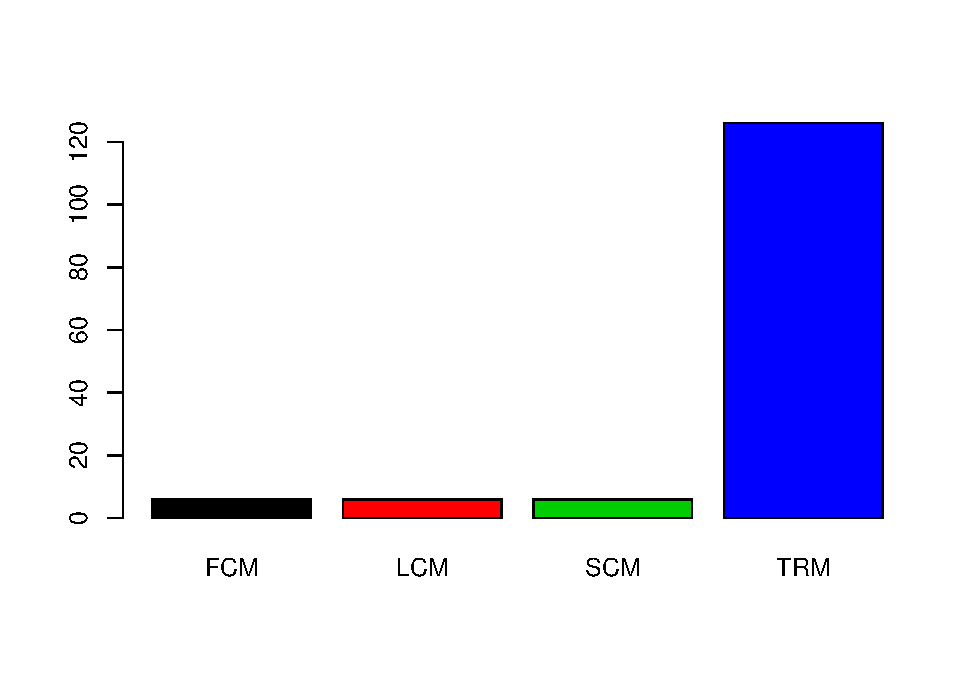
\includegraphics{./tex2pdf.8500/43a41a44ca93297326380ebb308b4fd130fa6906.pdf}

\begin{Shaded}
\begin{Highlighting}[]
\KeywordTok{show}\NormalTok{(rB)}
\end{Highlighting}
\end{Shaded}

\begin{verbatim}
##      [,1]
## [1,]  0.7
## [2,]  1.9
## [3,]  3.1
## [4,]  4.3
\end{verbatim}

\subsubsection{Table of Rivers Crossed With
Species}\label{table-of-rivers-crossed-with-species}

\begin{Shaded}
\begin{Highlighting}[]
\NormalTok{rsT <-}\StringTok{ }\KeywordTok{with}\NormalTok{(ddt, }\KeywordTok{table}\NormalTok{(RIVER, SPECIES))}
\KeywordTok{show}\NormalTok{(rsT)}
\end{Highlighting}
\end{Shaded}

\begin{verbatim}
##      SPECIES
## RIVER CCATFISH LMBASS SMBUFFALO
##   FCM        6      0         0
##   LCM        6      0         0
##   SCM        6      0         0
##   TRM       78     12        36
\end{verbatim}

\subsubsection{Barplot of Rivers Crossed With
Species}\label{barplot-of-rivers-crossed-with-species}

\begin{Shaded}
\begin{Highlighting}[]
\NormalTok{rcsB <-}\StringTok{ }\KeywordTok{barplot}\NormalTok{(rsT, }\DataTypeTok{beside=}\OtherTok{TRUE}\NormalTok{, }\DataTypeTok{col=}\DecValTok{1}\OperatorTok{:}\DecValTok{4}\NormalTok{)}
\end{Highlighting}
\end{Shaded}

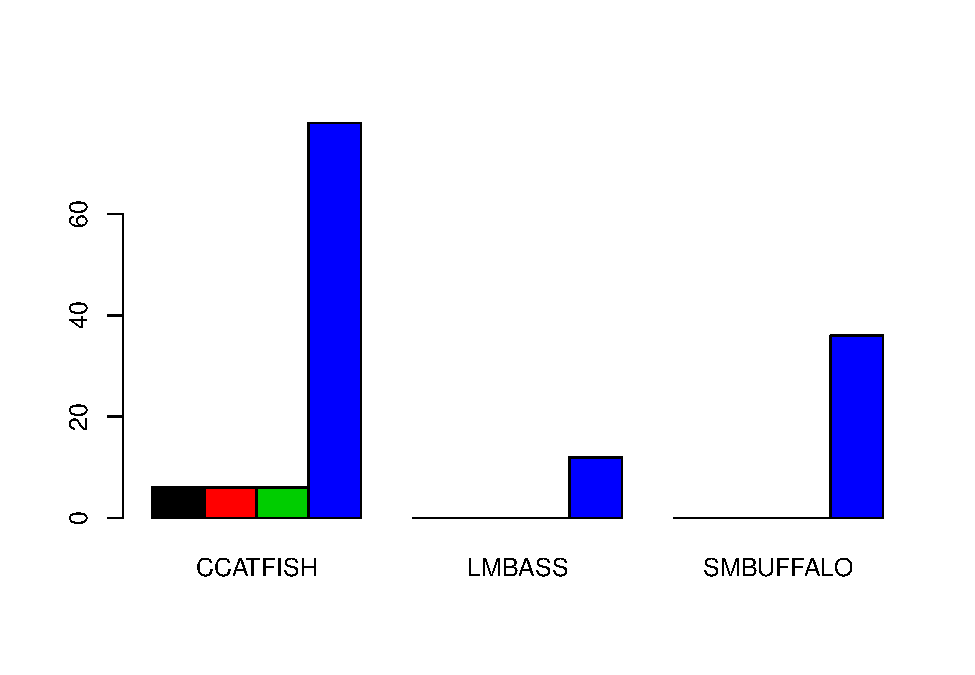
\includegraphics{./tex2pdf.8500/6eefa40cd5347852e59d3e6edaccd4b2c80d30ee.pdf}

\begin{Shaded}
\begin{Highlighting}[]
\KeywordTok{show}\NormalTok{(rcsB)}
\end{Highlighting}
\end{Shaded}

\begin{verbatim}
##      [,1] [,2] [,3]
## [1,]  1.5  6.5 11.5
## [2,]  2.5  7.5 12.5
## [3,]  3.5  8.5 13.5
## [4,]  4.5  9.5 14.5
\end{verbatim}

\subsection{Task 5}\label{task-5}

\subsubsection{PieCharts of Species and
Rivers}\label{piecharts-of-species-and-rivers}

\begin{Shaded}
\begin{Highlighting}[]
\NormalTok{sT <-}\StringTok{ }\KeywordTok{with}\NormalTok{(ddt, }\KeywordTok{table}\NormalTok{(SPECIES))}
\KeywordTok{layout}\NormalTok{(}\KeywordTok{matrix}\NormalTok{(}\KeywordTok{c}\NormalTok{(}\DecValTok{1}\NormalTok{, }\DecValTok{2}\NormalTok{),}\DataTypeTok{nr=}\DecValTok{1}\NormalTok{,}\DataTypeTok{nc=}\DecValTok{2}\NormalTok{))}
\KeywordTok{pie}\NormalTok{(sT)}
\KeywordTok{pie}\NormalTok{(rT)}
\end{Highlighting}
\end{Shaded}

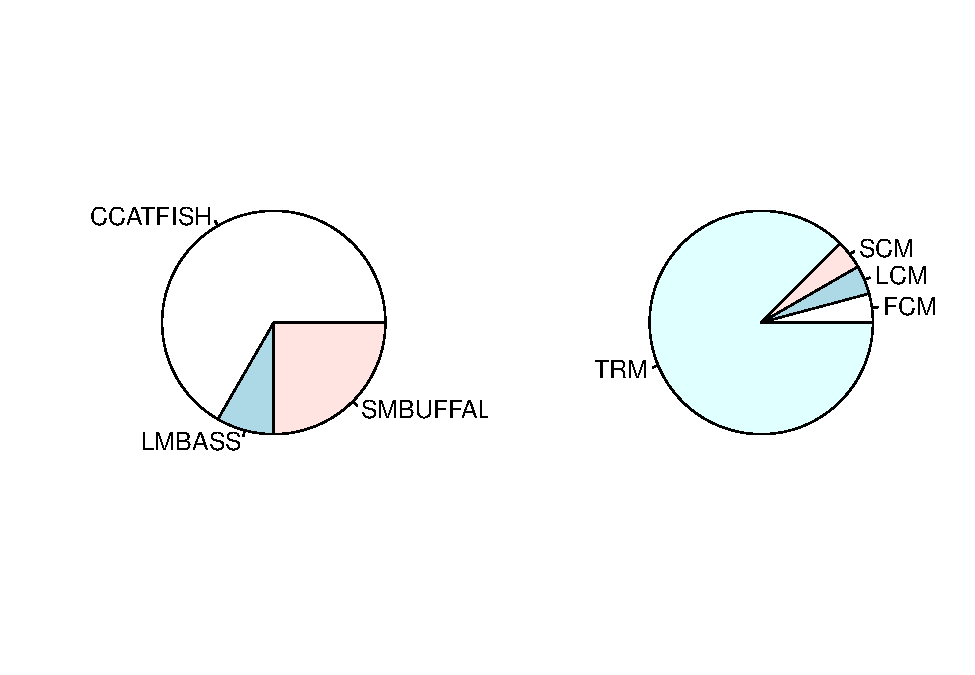
\includegraphics{./tex2pdf.8500/326cf2f84c38d68d6f6073cd225aaa2e488337a8.pdf}

\subsection{Task 6}\label{task-6}

\subsubsection{BoxPlots of DDT, Weight, and
Length}\label{boxplots-of-ddt-weight-and-length}

\begin{Shaded}
\begin{Highlighting}[]
\KeywordTok{layout}\NormalTok{(}\KeywordTok{matrix}\NormalTok{(}\KeywordTok{c}\NormalTok{(}\DecValTok{1}\NormalTok{,}\DecValTok{2}\NormalTok{,}\DecValTok{3}\NormalTok{),}\DataTypeTok{nr=}\DecValTok{1}\NormalTok{,}\DataTypeTok{nc=}\DecValTok{3}\NormalTok{))}
\KeywordTok{with}\NormalTok{(ddt,}\KeywordTok{boxplot}\NormalTok{(LENGTH,}\DataTypeTok{ylab=}\StringTok{"DDT"}\NormalTok{,}\DataTypeTok{col=}\StringTok{"Blue"}\NormalTok{,}\DataTypeTok{notch=}\OtherTok{TRUE}\NormalTok{))}
\KeywordTok{with}\NormalTok{(ddt,}\KeywordTok{boxplot}\NormalTok{(WEIGHT,}\DataTypeTok{ylab=}\StringTok{"WEIGHT"}\NormalTok{,}\DataTypeTok{col=}\StringTok{"Green"}\NormalTok{,}\DataTypeTok{notch=}\OtherTok{TRUE}\NormalTok{))}
\KeywordTok{with}\NormalTok{(ddt,}\KeywordTok{boxplot}\NormalTok{(MILE,}\DataTypeTok{ylab=}\StringTok{"LENGTH"}\NormalTok{,}\DataTypeTok{col=}\StringTok{"Red"}\NormalTok{,}\DataTypeTok{notch=}\OtherTok{TRUE}\NormalTok{))}
\end{Highlighting}
\end{Shaded}

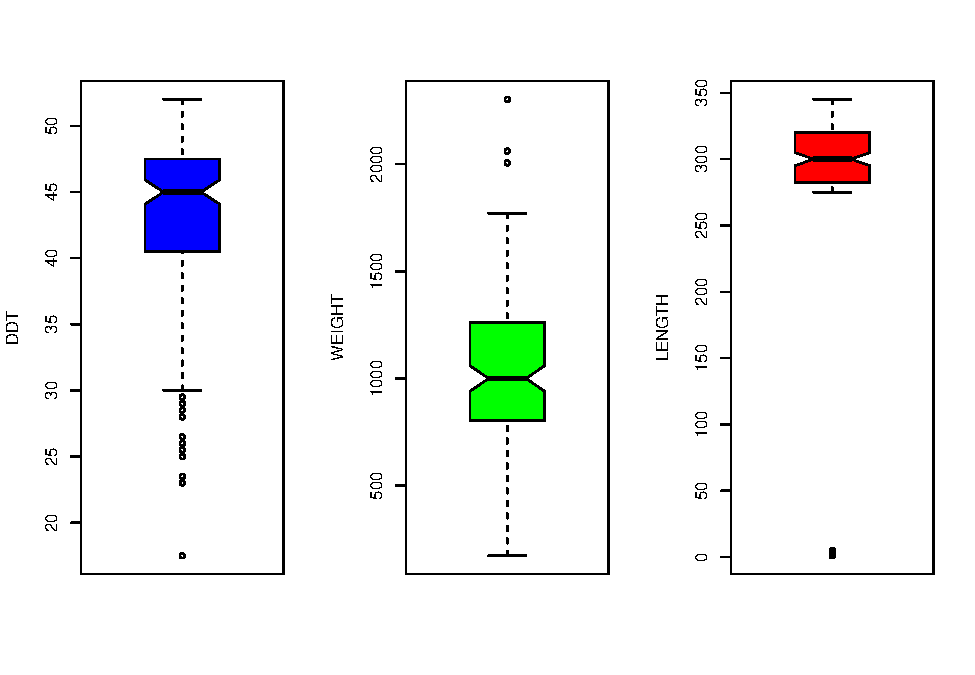
\includegraphics{./tex2pdf.8500/a3bacb5cbcb7dd6a84f7b2b31506186c6665033d.pdf}

\subsection{Task 7}\label{task-7}

\subsubsection{Coplot of Length V Weight Given
River}\label{coplot-of-length-v-weight-given-river}

\begin{Shaded}
\begin{Highlighting}[]
\NormalTok{lwC <-}\StringTok{ }\KeywordTok{coplot}\NormalTok{(LENGTH }\OperatorTok{~}\StringTok{ }\NormalTok{WEIGHT }\OperatorTok{|}\StringTok{ }\NormalTok{RIVER, ddt, }\DataTypeTok{col =} \DecValTok{1}\OperatorTok{:}\DecValTok{5}\NormalTok{)}
\end{Highlighting}
\end{Shaded}

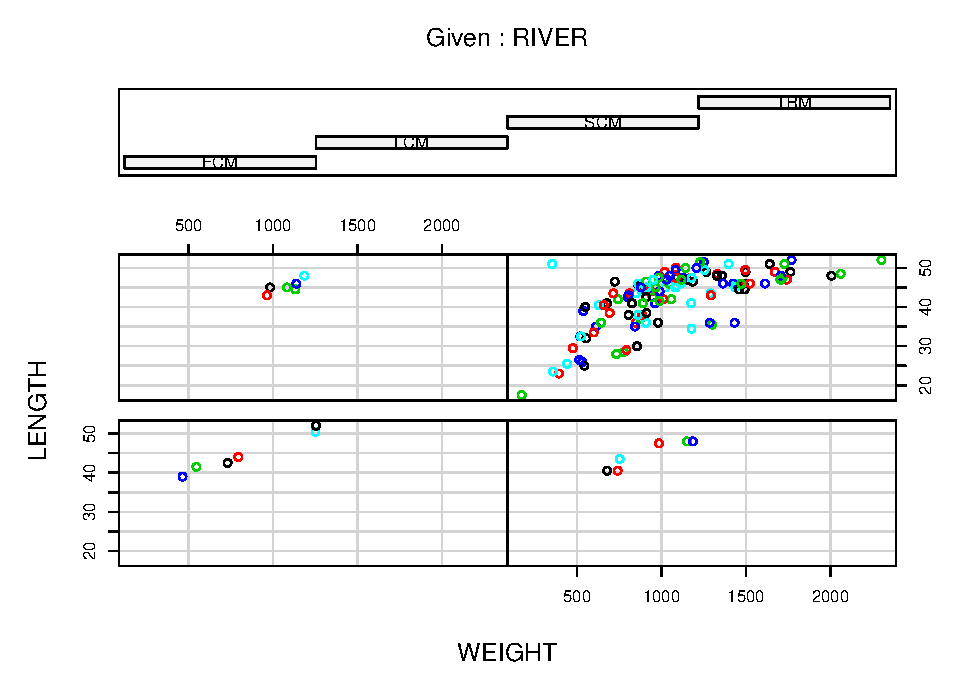
\includegraphics{./tex2pdf.8500/c8f018cad7f7fa434cf5387c68505ddc3c1d66e9.pdf}

\subsubsection{Coplot of DDT V Weight Given
Species}\label{coplot-of-ddt-v-weight-given-species}

\begin{Shaded}
\begin{Highlighting}[]
\NormalTok{dwC <-}\StringTok{ }\KeywordTok{coplot}\NormalTok{(DDT }\OperatorTok{~}\StringTok{ }\NormalTok{WEIGHT }\OperatorTok{|}\StringTok{ }\NormalTok{SPECIES, ddt, }\DataTypeTok{col =} \DecValTok{1}\OperatorTok{:}\DecValTok{4}\NormalTok{)}
\end{Highlighting}
\end{Shaded}

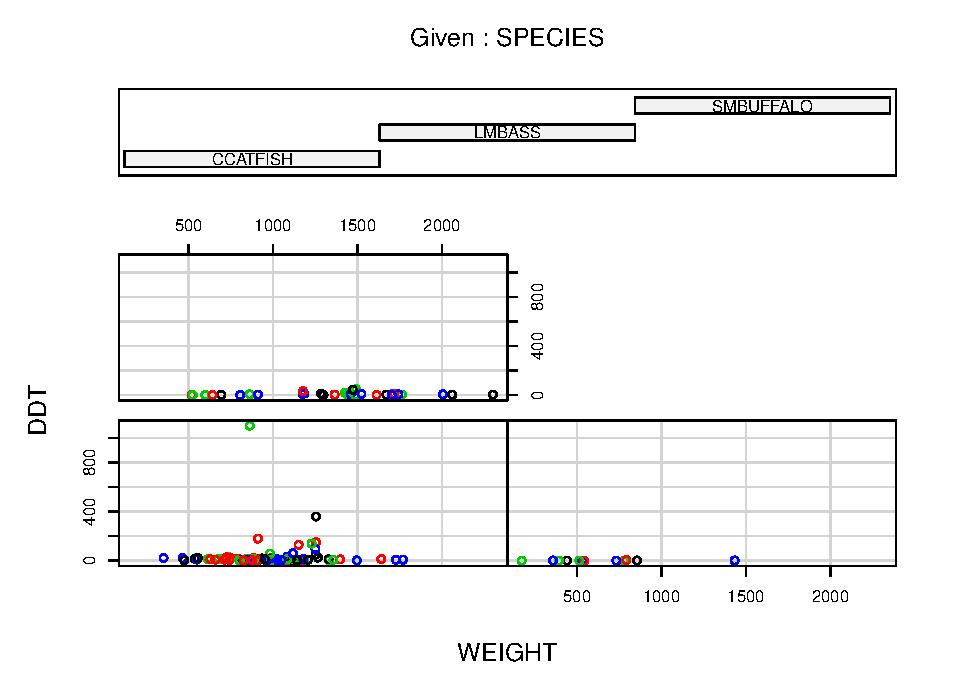
\includegraphics{./tex2pdf.8500/f9fd71bca2c34cce28a038add56edfa912c4976d.pdf}

\subsection{Task 8}\label{task-8}

\subsubsection{ggplot Box Plot Given Species and
Weight}\label{ggplot-box-plot-given-species-and-weight}

\begin{Shaded}
\begin{Highlighting}[]
\KeywordTok{library}\NormalTok{(ggplot2)}
\NormalTok{swgg <-}\StringTok{ }\KeywordTok{ggplot}\NormalTok{(ddt, }\KeywordTok{aes}\NormalTok{(}\DataTypeTok{x=}\NormalTok{SPECIES, }\DataTypeTok{y=}\NormalTok{WEIGHT, }\DataTypeTok{color=}\NormalTok{RIVER, }\DataTypeTok{fill =}\NormalTok{ RIVER))}
\NormalTok{swgg <-}\StringTok{ }\NormalTok{swgg }\OperatorTok{+}\StringTok{ }\KeywordTok{geom_boxplot}\NormalTok{(}\DataTypeTok{colour =} \StringTok{"#1F3552"}\NormalTok{)}
\NormalTok{swgg <-}\StringTok{ }\NormalTok{swgg }\OperatorTok{+}\StringTok{ }\KeywordTok{ggtitle}\NormalTok{(}\StringTok{"Clayton Glenn"}\NormalTok{)}
\KeywordTok{show}\NormalTok{(swgg)}
\end{Highlighting}
\end{Shaded}

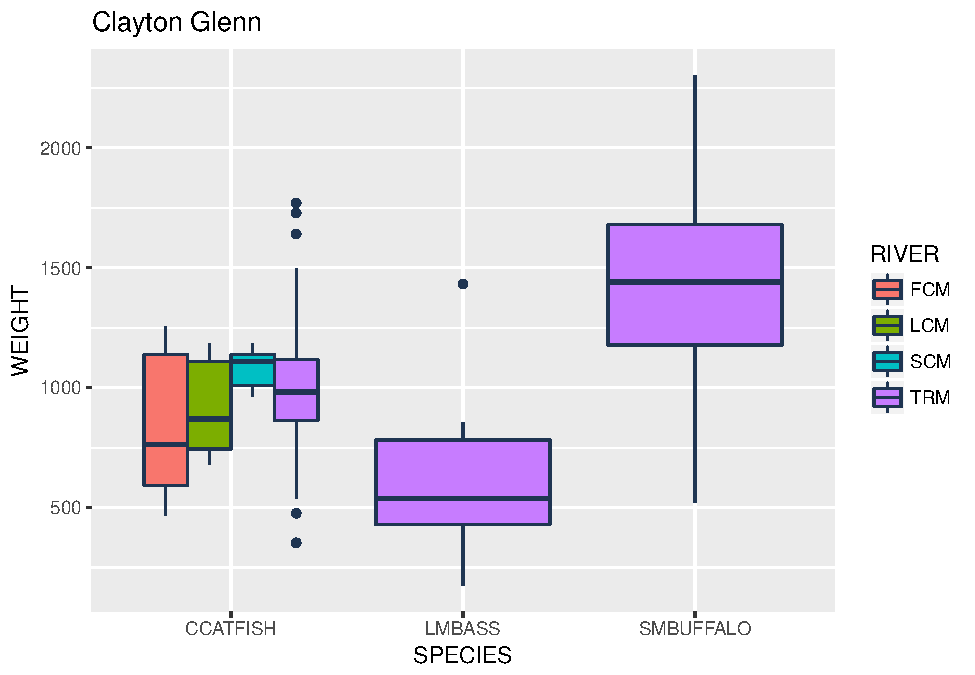
\includegraphics{./tex2pdf.8500/c3b6f01f5d7439085684a28b65a9926572c6b645.pdf}

\subsubsection{Violin Plot given River and
Length}\label{violin-plot-given-river-and-length}

\begin{Shaded}
\begin{Highlighting}[]
\KeywordTok{library}\NormalTok{(ggplot2)}
\NormalTok{rlgg <-}\StringTok{ }\KeywordTok{ggplot}\NormalTok{(ddt, }\KeywordTok{aes}\NormalTok{(}\DataTypeTok{x=}\NormalTok{RIVER, }\DataTypeTok{y=}\NormalTok{LENGTH, }\DataTypeTok{color=}\NormalTok{SPECIES, }\DataTypeTok{fill =}\NormalTok{ SPECIES))}
\NormalTok{rlgg <-}\StringTok{ }\NormalTok{rlgg }\OperatorTok{+}\StringTok{ }\KeywordTok{geom_violin}\NormalTok{(}\DataTypeTok{colour =} \StringTok{"#1F3552"}\NormalTok{)}
\NormalTok{rlgg <-}\StringTok{ }\NormalTok{rlgg }\OperatorTok{+}\StringTok{ }\KeywordTok{ggtitle}\NormalTok{(}\StringTok{"Clayton Glenn"}\NormalTok{)}
\KeywordTok{show}\NormalTok{(rlgg)}
\end{Highlighting}
\end{Shaded}

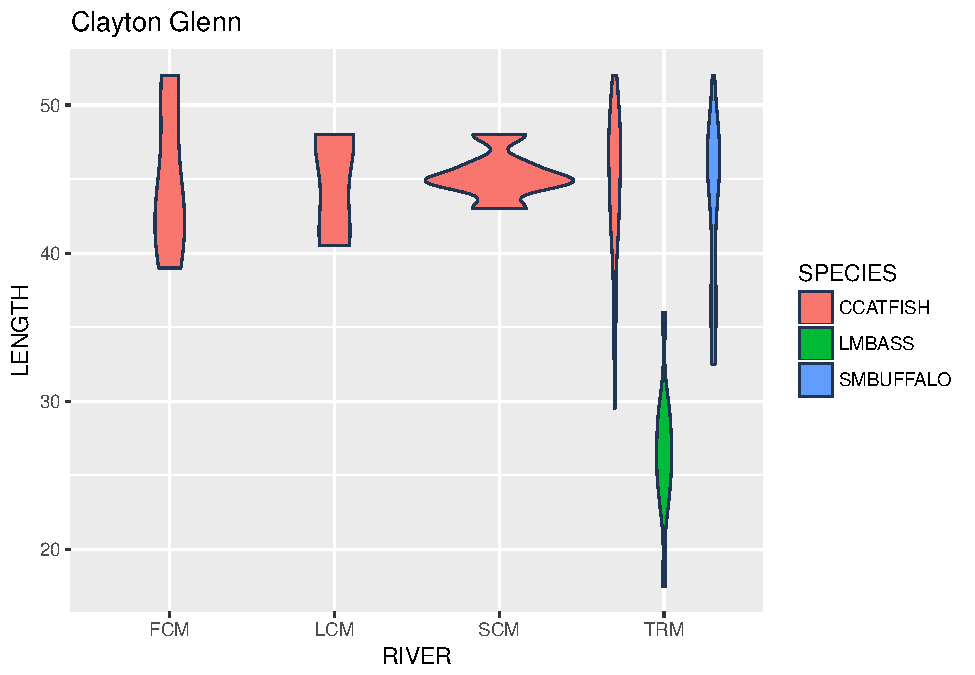
\includegraphics{./tex2pdf.8500/354dd74f754e16de8fdafbd827c1ccc2a98fc4d4.pdf}

\subsubsection{gg Scatter Plot given Weight and
Length}\label{gg-scatter-plot-given-weight-and-length}

\begin{Shaded}
\begin{Highlighting}[]
\KeywordTok{library}\NormalTok{(ggplot2)}
\KeywordTok{ggplot}\NormalTok{(ddt, }\KeywordTok{aes}\NormalTok{(}\DataTypeTok{x=}\NormalTok{WEIGHT, }\DataTypeTok{y=}\NormalTok{LENGTH, }\DataTypeTok{color=}\NormalTok{SPECIES, }\DataTypeTok{fill =}\NormalTok{ SPECIES)) }\OperatorTok{+}\StringTok{ }\KeywordTok{geom_point}\NormalTok{() }\OperatorTok{+}\StringTok{ }\KeywordTok{ggtitle}\NormalTok{(}\StringTok{"Clayton Glenn"}\NormalTok{)}
\end{Highlighting}
\end{Shaded}

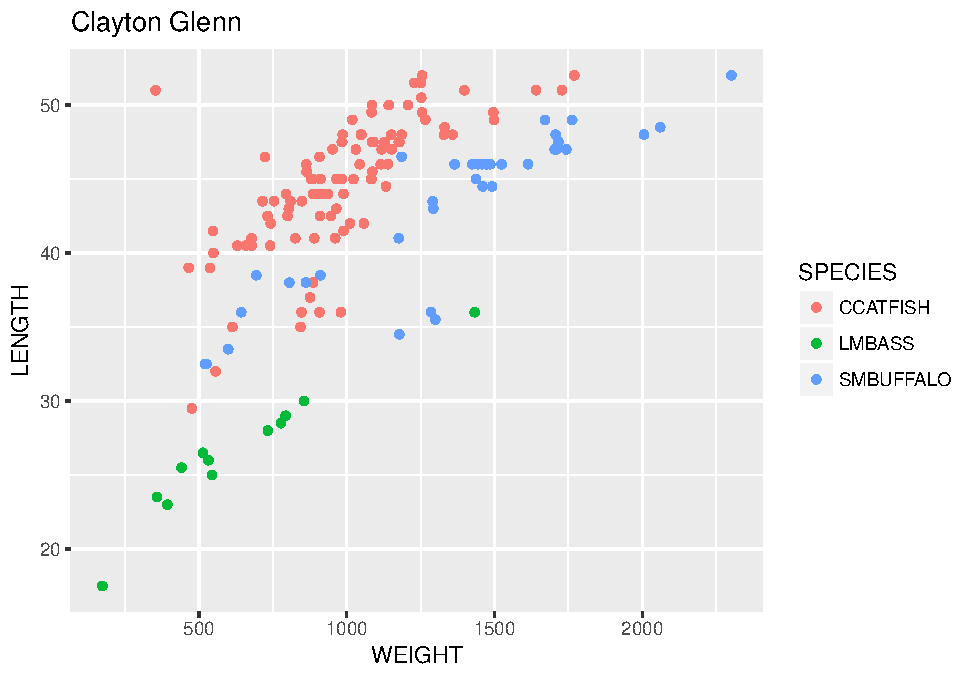
\includegraphics{./tex2pdf.8500/1992432b7d1bcbb7ffcb3d0766894b657da66071.pdf}

\section{Clicker Questions}\label{clicker-questions}

\subsection{Length Mean}\label{length-mean}

\begin{Shaded}
\begin{Highlighting}[]
\KeywordTok{mean}\NormalTok{(ddt}\OperatorTok{$}\NormalTok{LENGTH)}
\end{Highlighting}
\end{Shaded}

\begin{verbatim}
## [1] 42.8125
\end{verbatim}

\subsection{Weight Standard Deviation}\label{weight-standard-deviation}

\begin{Shaded}
\begin{Highlighting}[]
\KeywordTok{sd}\NormalTok{(ddt}\OperatorTok{$}\NormalTok{LENGTH)}
\end{Highlighting}
\end{Shaded}

\begin{verbatim}
## [1] 6.882093
\end{verbatim}


\end{document}
